\section{Introduction}\label{gen:sec:intro}

Inefficient queries are a significant problem for nearly any organization relying on a database system. These poorly written queries—whether authored by inexperienced users or auto-generated by business intelligence (BI) tools—are a major cause of slow performance and, in cloud databases like Snowflake~\cite{dageville2016snowflake} or BigQuery~\cite{fernandes2015bigquery}, can lead to excessive costs. 
As a result, SQL-to-SQL query rewriting is a crucial step in optimizing performance and reducing expenses, 
as the likelihood of the query optimizer finding an efficient query plan is significantly diminished if it is given a poorly-written query to begin with. 
However, whether performed manually or automatically, query rewriting has remained a challenging task.

\genhead{Challenges of manual query rewriting}
The poorly-written queries that have the biggest impact on the overall cost and performance tend to be quite complex too. 
For example, it is not uncommon for queries auto generated by
Looker~\cite{lookergoogle} to span 100s of lines.
Ensuring the rewritten query preserves the semantics of the original requires a deep understanding of the database schema, constraints, and the user intent, and is therefore a time-consuming and error-prone task, even for seasoned database experts.
The fact that there are often thousands, if not millions, of such slow queries makes the manual approach a monumental undertaking.

\genhead{Limitations of traditional automated query rewriting} 
Despite extensive research, automated query rewriting techniques have long faced fundamental limitations that hinder their practical effectiveness. The most common approach relies on \emph{rewrite rules}—--pattern-matching transformations that replace query fragments with optimized equivalents while preserving semantics. 
Regardless of whether the rules are developed and provided by experts~\cite{bruno2022computation,pirahesh1992extensible,ahmed2006cost} or 
are inferred automatically~\cite{wetune,ding2023proving},
a rule-based query rewriter is as effective as the set of rules provided to it. 
By definition, rule-based query rewriters\footnote{Rule-based query \emph{rewriting} should not be confused with rule-based query \emph{optimization}; the latter is simpler, and thus much more common in practice~\cite{graefe1987rule}.}
% are limited to situations where the input query matches one of their existing rules,  
% and thus
are fundamentally incapable of optimizing new query patterns that do not match their existing rules~\cite{dong2023slabcity}.
Although synthesis-based query-rewriting does not require prior rules~\cite{dong2023slabcity}, in practice it only handles simple queries---for instance, SlabCity~\cite{dong2023slabcity} optimizes just 2 out of 22 TPC-H~\cite{tpch} queries and 3 out of 99 TPC-DS~\cite{tpcds} queries.



\begin{comment}

\begin{table*}[htbp]
\centering
\label{gen:tab:plan_templates}
\begin{tabular}{|c|c|c|c|}
\hline
\textbf{No.} & \textbf{Source Query Pattern} & \textbf{Destination Query Pattern} & \textbf{Constraints} \\
\hline
1 & $\operatorname{Sel}_{\mathrm{p}, \mathrm{r} . \mathrm{a}_0}(\operatorname{Proj}_{\mathrm{r} . \mathrm{a}_1}(\mathrm{r}))$ & $\operatorname{Proj}_{\mathrm{r} . \mathrm{a}_1}(\operatorname{Sel}_{\mathrm{p}, \mathrm{r} . \mathrm{a}_0}(\mathrm{r}))$ & $\operatorname{SubAttrs}(a_0, a_1)$ \\
\hline
2 & $\operatorname{Proj}_{\mathrm{r} . \mathrm{a}_0}(\operatorname{Sel}_{\text {p,r. } \mathrm{a}_1}(\text { Proj }_{\mathrm{r} . \mathrm{a}_2}(\mathrm{r})))$ & $\operatorname{Proj}_{\mathrm{r} . \mathrm{a}_0}(\operatorname{Sel}_{\mathrm{p}, \mathrm{r} . \mathrm{a}_1}(\mathrm{r}))$ & $\operatorname{SubAttrs}(a_0, a_2), \operatorname{SubAttrs}(a_1, a_2)$ \\
\hline
3 & $\text { LJoin }_{\mathrm{r}_0, \mathrm{a}_0, \mathrm{r}_1 \cdot \mathrm{a}_1}(\mathrm{r}_0, \mathrm{r}_1)$ & $\text { IJoin }_{\mathrm{r}_0 \cdot \mathrm{a}_0, \mathrm{r}_1 \cdot \mathrm{a}_1}(\mathrm{r}_0, \mathrm{r}_1)$ & $\operatorname{RefAttrs}(\mathrm{r}_0, \mathrm{a}_0, \mathrm{r}_1, \mathrm{a}_1), \operatorname{NotNull}(\mathrm{r}_0, \mathrm{a}_0)$ \\
\hline
\end{tabular}
\caption{Examples of rewrite rules in WeTune~\cite{??}}
\end{table*}



\begin{enumerate}
    \item \textbf{Semantic side}: Ensuring that the rewrite preserves the semantics of the original query is crucial, which requires a deep understanding of the database schema, constraints, and the query intent.
    \item \textbf{Syntax side}: SQL queries and database schemas can be both highly complex. Manipulating their elements without introducing errors requires sophisticated analysis.
\end{enumerate}
\end{comment}

% \genbarzan{use either Text-to-SQL or Natural Language to SQL (NL2SQL) consistently everywhere in the paper}

% a few other 
% \genbarzan{would be better to name those areas here and cite them, e.g., blah~\cite{`}, blah~\cite{} and blah~\cite{}}
% areas~\cite{citeALlOtherPapersThatHaveAppliedLLMsToADBProblemExceptTheTextToSQLAndTheVisionPaperYouSentLastNight}, 

\genhead{Large language models (LLMs)} The shining success of large language models (LLMs) in performing complex and open-ended tasks has created new hopes for solving some of the hardest database problems as well. 
While researchers have used LLMs for Text-to-SQL~\cite{fu2023catsql,gao2023text,sun2306sql,katsogiannis2023survey,pourreza2024din} and a few other areas, e.g., data cleaning and integration~\cite{narayan2022can,suhara2022annotating}, table processing~\cite{li2023table,lu2024large} and database diagnosis~\cite{zhou2023d}, their potential for query rewriting has remained largely unexplored. In instances where human experts or existing rules cannot rewrite a query, say for complex queries or new query patterns, 
 could LLMs be leveraged to uncover rewrite opportunities due to their broad general knowledge and advanced reasoning capabilities? If so, this could drastically lower the burden on human experts and allow for a much larger set of queries to benefit from rewriting.
To the best of our knowledge, this paper is the first\footnote{See \S\ref{gen:sec:related} for related work published after the initial publication of our work on ArXiv.} to focus on 
 answering this question: how to best leverage LLMs for query rewriting beyond rules and how to address the challenges involved.

\genhead{Challenges} Using LLMs for query rewriting has challenges:\footnote{A common misunderstanding is that the time and monetary overhead of invoking an LLM may outweigh the speedup benefits of the rewrite. However, this one-time overhead is less relevant for repetitive workloads, which are the focus of \genrewrite (see \textbf{Target workloads}).} 
\begin{enumerate}[label=C\arabic*, leftmargin=0.5cm]

\item The na\"ive  approach of simply prompting the LLM to "rewrite the given query into a faster but equivalent form"  can rarely handle complex queries: 
most outputs either fail to parse (syntactic errors) or produce incorrect results (semantic errors) due to SQL’s complexity and LLM hallucinations (\S~\ref{gen:sec:expr:llmbaseline}).
%~\cite{zhang2023siren,tonmoy2024comprehensive}.

\item LLMs lack a database cost model and cannot run experiments, so their rewrites are not necessarily faster than the original queries.

\item While LLM costs for rewriting a recurrent workload can be amortized, excessive invocations can still become expensive.
     
\item Hints can help the LLM, but excessive or irrelevant ones can lead to mistakes.

\item Due to their black-box nature, LLM rewrites are harder for humans to understand and verify than traditional  rules.

\end{enumerate}

%ta inja
\genhead{Our approach}
To address the above challenges, we present \textbf{\genrewrite}, the first holistic system that leverages LLMs for query rewriting. 
We introduce the notion of a Natural Language Rewrite Rule (NLR2), which is a textual explanation summarizing the rewrite. 
We use the LLM itself to produce the NLR2s, which are then used for three purposes. The NLR2s 1)  serve as hints assisting the LLM to provide better rewrites 
(C2), requiring fewer follow-up LLM invocations (C4), 2) make the rewrites easier to understand and verify by offering a human-readable explanation (C5), and, 
most importantly, 3) allow \genrewrite to transfer the knowledge gained from rewriting one query to another and thus become smarter and more effective over time (C1, C2, C3). Since NLR2s are void of confidential information (such as column or schema names), one can even bootstrap \genrewrite's NLR2 repository for a new workload using the repository of a previously trained \genrewrite on another workload.

To avoid redundant rules, which can in turn confuse the LLM, we maintain
    a utility score for each NLR2 to supply only those rules to the LLM  as hints that are most relevant to the query at hand.
Finally, to minimize the LLM cost and minimize the human effort needed for manual verification, 
\genrewrite does not discard incorrect rewrites. Instead, it uses a novel counterexample-guided technique to iteratively
    correct the syntactic and semantic errors in the rewritten query (C1, C3).

\begin{figure}[ht]
\inv\sinv
  \centering
  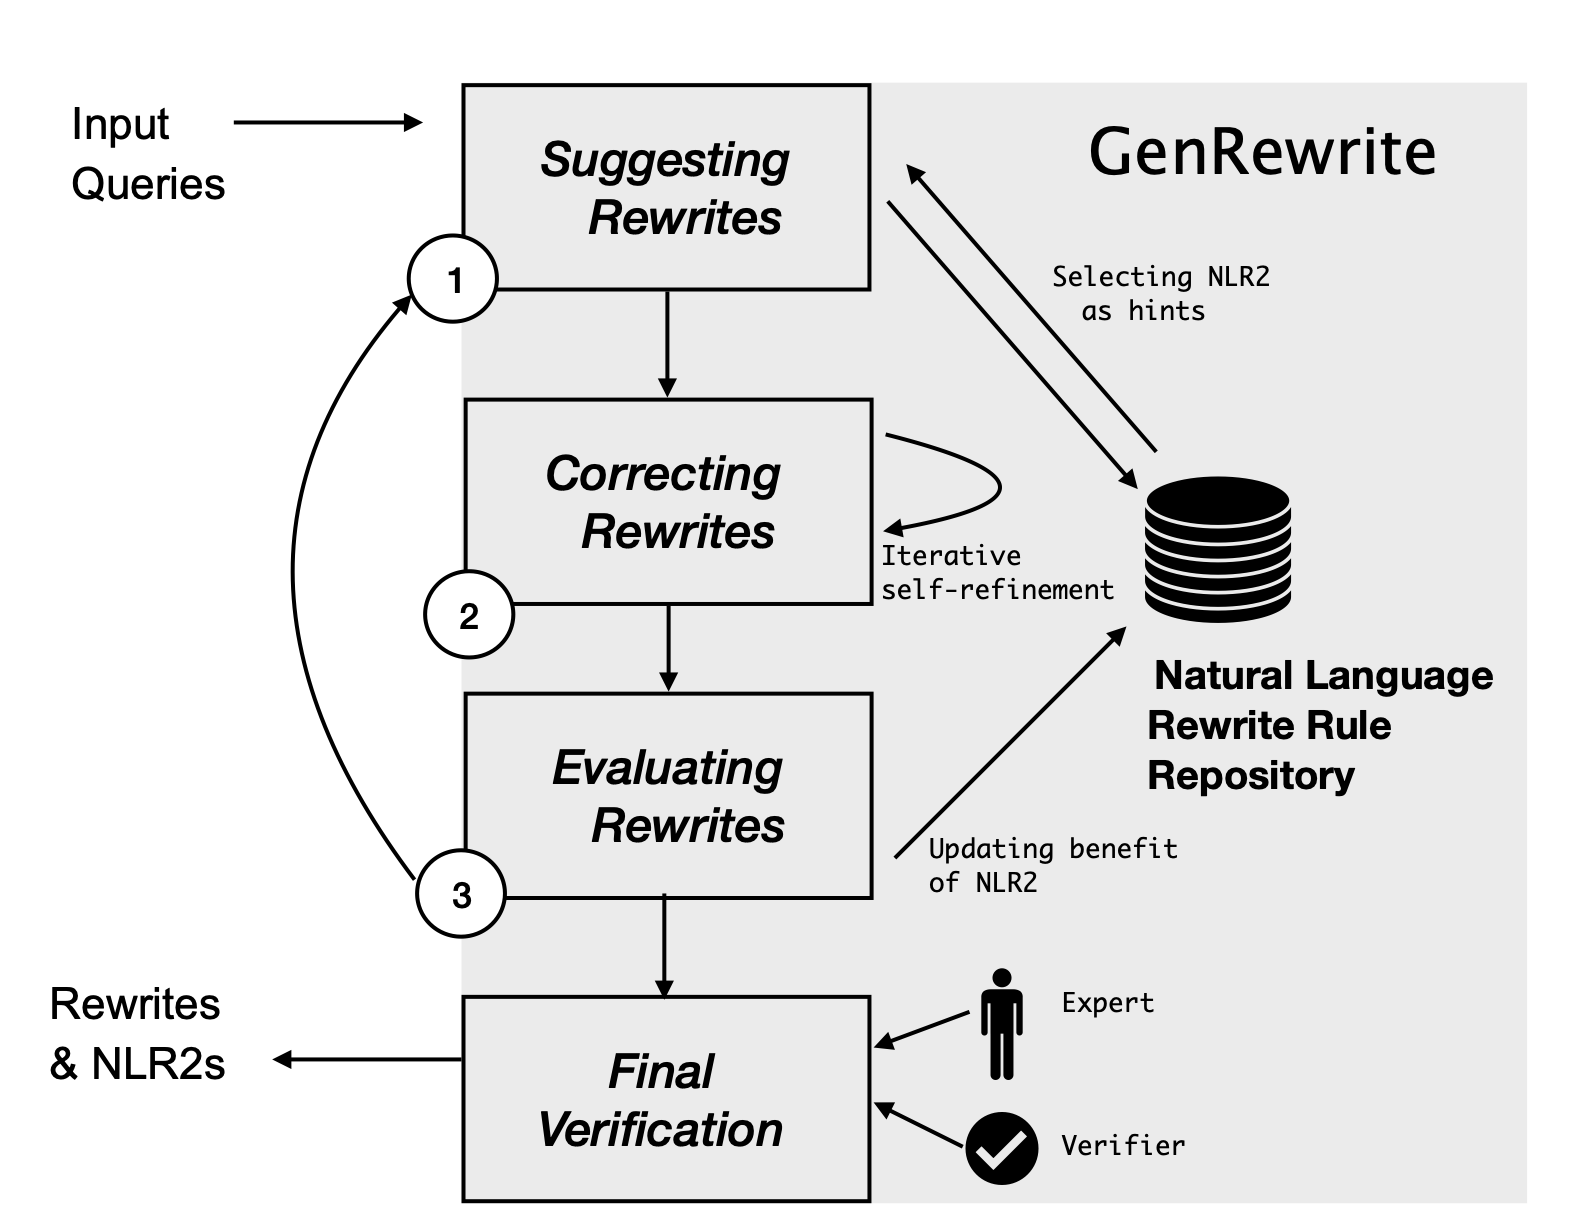
\includegraphics[width=0.8\linewidth]{chapters/genrewrite/figures/workflow.1.png}
\inv\inv
  \caption{High-level Workflow of \genrewrite }
  \label{gen:fig:arch}
\inv
\end{figure}

% \genbarzan{don't forget to fix the plot. sent you a bunch of feedback on this yesterday} \genjie{btw it is really easy to get lost in voice msgs on whatsapp, could you please remind me of the problems of this figure if you still remember}


\genhead{High-level workflow} 
\genrewrite takes as input a workload,\footnote{A streaming setting is a special case, whereby queries are presented and rewritten one at a time.}
expressed as a set of input queries $\mathcal{Q}$, and returns
\{($q$,$q'$,$e$) \textbar  $q$ $\in$ $\mathcal{Q}_{opt}$ \}, where
  $\mathcal{Q}_{opt}\subseteq \mathcal{Q}$ is the optimizable subset of the input queries, 
  $q'$ is the rewritten query that is equivalent to $q$ but likely to run faster, and $e$ is 
 a human-readable explanation of the rewrite.
Figure~\ref{gen:fig:arch} shows the overall workflow, which is an iterative process.
In each iteration, every query in the workload goes through three phases to find a better rewrite than the one found in previous iterations:
{\small \Circled{1}}  rewrite suggestion, {\small \Circled{2}}  rewrite correction, and {\small \Circled{3}}  rewrite evaluation. 
Additionally, \genrewrite \revthree{maintains} a Natural Language Rewrite Rule (NLR2) repository for knowledge transfer across queries in the workload.
{\small \Circled{1}} selects appropriate NLR2s from the repository to serve as hints for suggesting new rewrites. Any newly discovered NLR2 is also added to the repository. 
{\small \Circled{2}} iteratively refines rewrites based on the counterexamples provided by the LLM  to eliminate semantic and syntactic errors.
  {\small \Circled{3}} evaluates the rewrites for equivalence and performance, and updates the benefit score of the used NLR2s accordingly.
This process continues until no additional improvement is found and the set of rewrites stabilizes. 
The rewrites then go through a final verification step {\small \Circled{4}}, 
where if the formal verifier cannot guarantee equivalence automatically,
a human expert is asked to manually inspect and confirm  the rewritten query's equivalence before it is used or deployed to production.

% \genjie{yes, this module asks for counterexamples; I will mention it. The output from (2) is what LLMs believe are correct. There may be a gap between what LLMs believe are correct and what are actually correct. So we can add a correctness checking module in (3). (3) checks equivalence and speedups at the same time.}


\genhead{Target workloads} Repeatedly invoking an LLM incurs a time and monetary overhead. 
% For instance, \genrewrite uses a default budget of 45 seconds that can be adjusted by users. 
 As mentioned above, when the formal verifier cannot guarantee the equivalence, a human expert needs to inspect the rewrite, which incurs an additional delay.
 For these reasons, \genrewrite is only focused on the following use cases:
\begin{enumerate}[leftmargin=0.5cm]
\item \textbf{Recurrent workloads}, where the same query template is executed many times, such as BI (Business Intelligence) dashboards, reporting, ETL, DB-based applications, and dbt~\cite{dbt} jobs. 
For instance, 
over 60\% of the jobs in Microsoft clusters are recurrent~\cite{jindal2018selecting}.
Here, queries can be rewritten and optimized by \genrewrite once and then reused many times.

\item \textbf{Highly expensive queries} expected to take 10s of minutes, e.g., an adhoc query scanning terabytes of data.
Here, even if the query is run once, the additional overhead of leveraging an LLM or a human expert is still well justified.
\end{enumerate}

 In other words, \genrewrite is \emph{not} designed for real-time adhoc workloads, where queries are novel \textbf{\underline{and}} relatively light, as the additional overhead of an LLM cannot be amortized.
 


\genhead{Contributions} We make the following contributions:
\begin{enumerate}[leftmargin=0.5cm]
    \item We present one of the first in-depth analyses of LLMs for query rewriting, outlining key challenges and opportunities for future research in this area (\S\ref{gen:sec:insight}).
    \item We present \genrewrite, a holistic tool leveraging LLMs for autonomous query rewriting. It 
        addresses the key challenges of using LLMs by introducing (i) the notion of Natural Language Rewrite Rules (NLR2) for finding better rewrites and effective knowledge transfer,
          (ii)  a utility score for NLR2s to minimize LLM confusion caused by irrelevant or too many rules , and (iii) a counterexample-guided iterative correction method.
        (\S\ref{gen:sec:approach}).
    \item We evaluate \genrewrite on the standard TPC-DS and JOB benchmarks and \revtwo{their SQLStorm-generated variants}. \genrewrite consistently optimizes more queries at every speedup threshold than all baselines. \revtwo{At the $\geq$2x threshold on TPC-DS, \genrewrite improves 25 queries—~1.35x more than LLM-driven baselines and ~2.6x more than LLM-enhanced rule-based baselines—and the gap widens further on TPC-DS (SQLStorm); on JOB and its SQLStorm variant, where queries are simpler, absolute gains are smaller but \genrewrite still leads.} (\S\ref{gen:sec:expr}).
       
\end{enumerate}


% \revtwo{Across the standard TPC-DS and JOB benchmarks and their SQLStorm-generated variants~\cite{schmidt2025sqlstorm}, \genrewrite consistently optimizes more queries at every speedup threshold than both baseline categories. At the $\geq$2x threshold on TPC-DS, \genrewrite improves 25 queries—~1.35x more than LLM-driven baselines and ~2.6x more than LLM-enhanced rule-based baselines—and the gap widens further on TPC-DS (SQLStorm); on JOB and its SQLStorm variant, where queries are simpler, absolute gains are smaller but \genrewrite still leads.}

%  speeding up 25 out of 99 TPC-DS queries by more than 2x, which is  2.5x--4.2x higher coverage than state-of-the-art rule-based query rewriting and 1.4x higher than the out-of-the-box LLM performance.  


% 2.5x--3.2x higher coverage 
% over baselines 

% Furthermore, we conduct an ablation study to dissect how each component of \genrewrite contributes to its overall effectiveness. 



% Examples of rewrite rules include predicate pushdown, expression rewriting, and subquery unnesting.

% Large Language Models (LLMs) have made remarkable progress, excelling in understanding natural language and producing insightful responses.
 % Although LLMs are widely employed in Text-to-SQL solutions,
 % achieving knowledge transfer with Natural Language (NL) rewrite rules and largely solve the second the challenge by introducing a counterexample-guided iterative correction approach.

 % Our motivating use case is any scenario where the same  query is written once but rerun many times, such as BI dashboards. While GenRewrite’s budget can be specified by users, in this work we use at most 55 API calls. This cost is well justified by the observation that business-critical jobs in analytics clusters are typically recurrent, where instances of the same job are issued periodically over new batches of data, e.g., hourly, daily, or weekly. In fact, over 60\% of the jobs in Microsoft clusters are recurrent, with the majority of them being submitted daily. In such cases, users can invoke GenRewrite as a final step to identify any optimizations before running the workload, leveraging GenRewrite's advanced query rewriting capabilities to minimize execution time and resource consumption.